\documentclass[8pt,a4paper]{article}

\usepackage{amsmath}
\usepackage{tikz}
\usepackage{amssymb}
\usepackage{multicol}
\usepackage[top=0.5cm,left=0.5cm,right=0.5cm,bottom=0.5cm]{geometry}
\usepackage{amsfonts}
\usepackage{etoolbox}
\usepackage{cancel}
\usepackage{yhmath}

\newcommand{\EE}{\mathbb E}
\newcommand{\NN}{\mathbb N}
\newcommand{\PP}{\mathbb P}
\newcommand{\RR}{\mathbb R}
\newcommand{\ZZ}{\mathbb Z}

\newcommand{\Ac}{\mathcal A}
\newcommand{\Bc}{\mathcal B}
\newcommand{\Cc}{\mathcal C}
\newcommand{\Ec}{\mathcal E}
\newcommand{\Fc}{\mathcal F}
\newcommand{\Gc}{\mathcal G}
\newcommand{\Hc}{\mathcal H}
\newcommand{\Lc}{\mathcal L}
\newcommand{\Nc}{\mathcal N}
\newcommand{\Pc}{\mathcal P}

% d nell'integrale
\newcommand{\de}{\mathrm d}
\newcommand{\dx}{\de x}
\newcommand{\dy}{\de y}
\newcommand{\dP}{\de P}
\newcommand{\dPP}{\de \PP}

\newcommand{\Bot}{\perp \!\!\! \perp} % indipendenza
\usepackage{dsfont} % per funzione indicatrice
\newcommand{\Ind}{\mathds{1}} % funzione indicatrice

\DeclareMathOperator{\MCD}{MCD}
\DeclareMathOperator{\Det}{det} % determinante
\DeclareMathOperator{\Var}{Var} % varianza
\DeclareMathOperator{\Cov}{Cov} % covarianza
\DeclareMathOperator{\Img}{Im}
\DeclareMathOperator{\Col}{Col}
\DeclareMathOperator{\Ker}{Ker}
\DeclareMathOperator{\Bi}{Bi} % binomiale
\DeclareMathOperator{\Be}{Be} % bernoulli

% per far essere piccoli sum e prod
\makeatletter
\newcommand{\changeoperator}[1]{%
  \csletcs{#1@saved}{#1@}%
  \csdef{#1@}{\changed@operator{#1}}%
}
\newcommand{\changed@operator}[1]{%
  \mathop{%
    \mathchoice{\textstyle\csuse{#1@saved}}
               {\csuse{#1@saved}}
               {\csuse{#1@saved}}
               {\csuse{#1@saved}}%
  }%
}
\makeatother

\changeoperator{sum}
\changeoperator{prod}
 
 % Turn off header and footer
\pagestyle{empty}

% Redefine section commands to use less space
\makeatletter
\renewcommand{\section}{\@startsection{section}{1}{0mm}%
                                {-0.1ex plus -.5ex minus -.2ex}%
                                {0.5ex plus .2ex}%x
                                {\normalfont\large\bfseries}}
\renewcommand{\subsection}{\@startsection{subsection}{2}{0mm}%
                                {0.7ex plus 0ex minus 0ex}%
                                {-2.1ex plus 0ex}%
                                {\normalfont\scriptsize\bfseries}}
\renewcommand{\subsubsection}{\@startsection{subsubsection}{3}{0mm}%
                                {-1ex plus -.5ex minus -.2ex}%
                                {1ex plus .2ex}%
                                {\normalfont\small\bfseries}}
\makeatother

%\titlespacing\section{0pt}{0pt plus 0pt minus 0pt}{0pt plus 0pt minus 0pt}

% Don't print section numbers
\setcounter{secnumdepth}{0}

\setlength{\parindent}{0pt}
\setlength{\parskip}{0pt plus 0ex}

% -----------------------------------------------------------------------

\begin{document}

\raggedright
\footnotesize
\begin{multicols}{3}

% multicol parameters
% These lengths are set only within the two main columns
%\setlength{\columnseprule}{0.25pt}
\setlength{\premulticols}{1pt}
\setlength{\postmulticols}{1pt}
\setlength{\multicolsep}{1pt}
\setlength{\columnsep}{2pt}

%!TEX root = foglio.tex

\subsection{Leggi di De Morgan:}

Sia $A_{\alpha} \subset \Omega $ famiglia di sottoinsiemi di $\Omega $ $( \cup_{\alpha} A_{\alpha})^C =\cap_{\alpha} A^C_{\alpha} ,( \cap_{\alpha} A_{\alpha})^C =\cup_{\alpha} A^C_{\alpha}$
\subsection{Funzione misurabile:}

Dati $(\Omega ,\Ac )$ e $(F,\Fc )$, una funzione $X:\Omega \rightarrow F$ è detta misurabile/variabile aleatoria se: $(X\in B)\in \Ac \ \ \forall B\in \Fc$
\subsection{Relazioni controimmagini-unioni, intersezioni o complementazioni}

$ \begin{array}{l}
X^{-1}\left( B^C\right) =\left( X^{-1} (B)\right)^C\\
X^{-1}( \cup_{\alpha} B_{\alpha}) =\cup_{\alpha} X^{-1}( B_{\alpha})\\
X^{-1}( \cap_{\alpha} B_{\alpha}) =\cap_{\alpha} X^{-1}( B_{\alpha})
\end{array}$
\subsection{Probabilità di un intervallo:}

$ \begin{array}{l}
P((x,y]) = F(y)   - F(x)   \\
P([x,y]) = F(y)   - F(x^-) \\
P((x,y)) = F(y^-) - F(x)   \\
P([x,y)) = F(y^-) - F(x^-) \\
P(\{x\}) = F(x)   - F(x^-)
\end{array}$
\subsection{Quantile di ordine $\alpha $:}

$\begin{cases}
P( X\leq q_{\alpha}) \geq \alpha \\
P( X\geq q_{\alpha}) \leq 1-\alpha 
\end{cases} \Leftrightarrow \begin{cases}
P( X\leq q_{\alpha}) \geq \alpha \\
P( X< q_{\alpha}) \leq \alpha 
\end{cases} \Rightarrow \begin{cases}
F_X( q_{\alpha}) \geq \alpha \\
F_X( q_{\overline{\alpha}}) \leq \alpha 
\end{cases}$
\subsection{Definizione limsup, liminf:}

$ \begin{array}{l}
\liminf X_n =\lim_{n\rightarrow +\infty}(\inf_{m >n} X_m)\\
\limsup X_n =\lim_{n\rightarrow +\infty}\left(\sup_{m >n} X_m\right)
\end{array}$
\subsection{Spazi L}

Si ricorda che $L^1$ e $L^2$ sono spazi vettoriali.

$ \begin{array}{l}
X:\Omega \rightarrow R\ \text{V.A.R.} \in L^1 \Leftrightarrow \EE[X]\in \RR\\
x\in L^1 \Leftrightarrow | x| \in L^1\\
X,Y\in L^p \ \text{e} \ X=Y\ \text{q.c.} \Leftrightarrow [X]=[Y]\in L^p
\end{array}$
\subsection{Cauchy-Schwarz:}

$ \begin{array}{l}
X,Y\in L^2 \Rightarrow \EE[XY]|\leq \sqrt{\EE\left[ X^2\right]\EE\left[ Y^2\right]}\\
X\in L^2 \Rightarrow \EE[X]^2 \leq \EE\left[ X^2\right]
\end{array}$
\subsection{Disuguaglianza di Markov:}

$X\ \text{V.A.R.} \Rightarrow P(|X|\geq a)\leq \frac{\EE[|X|]}{a} \ \ \forall a >0$
\subsection{Disuguaglianza di Chebychev:}

$X\in L^2 \ \text{V.A.R.} \Rightarrow P(| x-\mu | \geq a)\leq \frac{\Var(x)}{a^2}$
\subsection{Lemma di Fatou:}

Siano le VA $X_n$ e $Y$ tali che $X_n \geq Y$ qc, $Y\in \Lc^1$. Allora $\EE\left[\liminf_n X_n\right] \leq \liminf_n\EE[ X_n]$
\subsection{Tasso di fallimento: ($t >0$)}

$ \begin{array}{l}
h_X (t)=\lim_{\varepsilon \rightarrow 0^+}\frac{\PP (t< X< t+\varepsilon |X >t)}{\varepsilon}\\
h_X (t)=\frac{f_x (t)}{1-F_x (t)}
\end{array}$
\section{Valore atteso e momenti}
\subsection{Valore atteso:}

$\EE[h(X)]=\int_{\Omega} h(X(\omega ))I(d\omega )=\int_{\Omega} h(X(\omega ))P(d\omega )=\int_{\RR} h(x)P^X (\dx)=\int_{\RR} h(x)f_X (x)\dx$

Nel caso discreto: $\EE[h(x)]=\sum_k h( x_k) p_k$
\subsection{Varianza e covarianza:}

$ \begin{array}{l}
\Var(X)=\sigma^2_X =\EE\left[ X^2\right] -\EE[X]^2\\
\Cov(X,Y)=\sigma_{XY} =\EE[XY]-\EE[X]\EE[Y]\\
\Var(X+Y)=\Var(X)+\Var(Y)+2\Cov(X,Y)\\
\Var(aX+b) =a^2\Var X\\
\Cov(a,X) =0\\
\Cov(aX+bY,Z) =a\Cov(X,Z) +b\Cov(Y,Z)\\
\Cov(X,Y) =\rho \sigma_X \sigma_Y
\end{array}$
\subsection{Coefficiente di correlazione lineare:}

$\rho =\frac{\Cov(X,Y)}{\sqrt{\Var(X)\Var(Y)}}$
\subsection{Trasformazioni affini:}

Dato $Y=AX+b$, $\EE[Y]=A\EE[X]+b$, $\Var[Y]=A\Var[X]A^T =C_Y =AC_X A^T$
\section{Vettori aleatori}

Sia $X$ vettore aleatorio: $\EE[h(X)]=\int_{\Omega} h(X)d\PP =\int_{\RR^n} h(x)dP^X$

$=\begin{cases}
{\textstyle \sum\nolimits_{x\in S} h(x)p(x)} & X\text{ è discreto }\\
{\textstyle \int_{\RR^n} h(x)f(x)\dx} & X\text{ è continuo }
\end{cases}$

Per calcolare la funzione di ripartizione di una variabile specifica:

\textit{Continuo:} $f_k( x_k) =\int f( x_1 ,\dotsc ,n)\dx_1 \dotsc \dx_{k-1}\dx_{k+1} \dotsc \dx_n$ (integrale su tutte le componenti che non ci interessano, ovvero tutte tranne $x_k$)

\textit{Discreto:} gli integrali diventano sommatorie.

$X$ è un vett. al. continuo se $C$ è invertibile.
\subsection{Trasformazione vett. al. continuo}

Sia $(X,Y):\Omega \rightarrow \RR^2$ vett. al. continuo con densità $f_{(X,Y)}$. Il supporto di $P^{(X,Y)}$ è $S\subset \RR^2$. $(U,V)=h((X,Y))=( h_1 (X,Y),h_2 (X,Y))$ con $h:\RR^2\rightarrow \RR^2$. Se $h\in C^1 (S),\Det( J_h) (x,y)\neq 0$ e $\exists g=h^{-1} ,g:h(S)\rightarrow S$ con $g(u,v)=( g_1 (u,v),g_2 (u,v))$ allora $(U,V)$ è un vett. al. continuo e $f_{(U,V)} (u,v)=f_{( X,Y)}( g_1 (u,v),g_2 (u,v))| \Det( J_g) (u,v)| $
\section{Vettori aleatori gaussiani}

Dato $X=( X_1 ,\dotsc ,X_n) \sim \Nc (\mu ,C)$ dove $\mu \in \RR^n ,C\in \RR^{n\times n} ,C >0$, allora può anche essere definito come $\varphi_{( X_{1,\dotsc,n})} (u)=\exp\left\{i\left< u|\mu \right> -\frac{1}{2}\left< u|Cu\right> \right\} \Leftrightarrow \left< a|X\right> \sim \Nc \ \ \forall a\in \RR^n$ Quindi $f_X (x)=$

$\frac{1}{\sqrt{(2\pi )^n\Det (C)}}\exp\left\{-\frac{1}{2}\left< x-\mu |C^{-1} (x-\mu )\right> \right\}$
\subsection{Proprietà:}

1. $X_k \sim \Nc( \mu_k ,C_{kk})$

2. $S_X =\Img (C)+\mu =\Col (C)+\mu =[\Ker (C)]^{\perp} +\mu $

3. $X\ \text{Continuo} \Leftrightarrow \Det (C)\neq 0\Leftrightarrow C >0$

4. $X_i \Bot X_j \Leftrightarrow \Cov(X_i ,X_j) =0$

5. $X_i \sim \Nc\cancel{\Rightarrow} X\sim \Nc$, solo se sono anche $\Bot $
\subsection{Trasformazioni affini:}

$ \begin{array}{l}
Y=AX+b,\ \ Y\sim \Nc\left( A\mu +b,ACA^T\right)\\
X\sim \Nc\left( \mu_X ,\sigma^2_X\right) ,\ \ Y\sim \Nc\left( \mu_Y ,\sigma^2_Y\right)\\
aX+bY\sim \Nc\left( a\mu_X +b\mu_Y ,a^2 \sigma^2_X +b^2 \sigma^2_Y +2ab\sigma_{XY}\right)
\end{array}$

Da verificare: $a^2 \sigma^2_X +b^2 \sigma^2_Y +2ab\sigma_{XY} \geq 0$
\subsection{Caso bidimensionale:}

$\begin{bmatrix}
X\\
Y
\end{bmatrix} \sim \Nc\left(\begin{bmatrix}
\mu_X\\
\mu_Y
\end{bmatrix} ,\begin{bmatrix}
\sigma^2_X & \Cov(X,Y)\\
\Cov(X,Y) & \sigma^2_Y
\end{bmatrix}\right)$

$\varphi_{(X,Y)} (u,v)=\exp\left\{i( \mu_X u+\mu_Y v) -\frac{1}{2}\left( u^2 \sigma^2_X +2\sigma_{XY} uv+v^2 \sigma^2_Y\right)\right\}$

In questo caso la proprietà (3) può anche essere espressa come:

$\begin{bmatrix}
X\\
Y
\end{bmatrix} \ \text{Cont.} \Leftrightarrow \Det (C)\neq 0\Leftrightarrow \begin{cases}
\sigma_X >0\\
\sigma_Y >0\\
| \rho_{X,Y}| < 1
\end{cases}$

$f_{(X,Y)} (x,y)=\frac{1}{2\pi \sigma_X \sigma_Y\sqrt{1-\rho^2}}\exp\left\{-\frac{1}{2( 1-\rho^2 )}\right.$\\$\left.\left[\frac{( x-\mu_X)^2}{\sigma^2_X} -2\rho \frac{( x-\mu_X)( y-\mu_Y)}{\sigma_X \sigma_Y} +\frac{( y-\mu_y)^2}{\sigma^2_Y}\right]\right\}$
\section{Funzioni caratteristiche}

Funzione complessa in corrispondenza biunivoca con la legge, la quale è da essa caratterizzata. $\varphi_X (u)=\int_{\RR^n} e^{i\left< u|X\right>} P^X (\dx)=\EE\left[ e^{i\left< u|X\right>}\right] =\int_{\Omega} e^{i\left< u|X\right>} d\PP$
\subsection{Funzione caratteristica e momenti:}

$ \begin{array}{l}
\frac{\partial^m}{\partial u_{k1} \cdots \partial u_{km}} \varphi (0)=i^m\EE[ X_{k1} \cdots X_{km}]\\
\EE[ X_k] =\frac{1}{i}\frac{\partial \varphi (0)}{\partial u_k}\\
\EE\left[ X^2_k\right] =-\frac{\partial^2 \varphi (0)}{\partial u^2_k} ,\ \EE[ X_k X_j] =-\frac{\partial^2 \varphi (0)}{\partial u_k \partial u_j}
\end{array}$
\subsection{Trasformazioni affini:}

$Y=AX+b\Rightarrow \varphi_Y (u)=e^{i\left< u|b\right>} \varphi_X\left( A^T u\right)$
\section{Prob. e leggi condizionate}
\subsection{Probabilità condizionata:}

$ \begin{array}{l}
P(A|B)=\frac{P(A,B)}{P(B)}\\
P(A)=\sum_n P( A\cap E_n) =\sum_n P( A|E_n) P( E_n)
\end{array}$
\subsection{Formula di Bayes:}

$P( E_k |A) =\frac{P( A|E_k) P( E_k)}{\sum_n P( A|E_n) P( E_n)}$
\subsection{Leggi condizionate:}

$ \begin{array}{l}
Y|X=x\sim f_{Y|X} (\cdot |x)\\
f_{(X,Y)} (x,y)=f_{(Y|X)} (y,x)\cdot f_X (x)\\
\EE[Y|X=x]=m(x)=\int_{S_Y} yf_{Y|X} (y,x)dy
\end{array}$

$\Var(Y|X=x)=q^2 (x)=\int_{S_Y} (y-m(x))^2 f_{Y|X} (y,x)dy$

Nel caso di VA discrete è sufficiente sostituire $P$ ad $f$ e svolgere gli integrali come sommatorie.
\subsection{Valore atteso condizionato:}

Se $Y\in L^1$ allora $\EE[Y]=\EE[\EE[Y|X]]$
\subsection{Varianza condizionata:}

$\Var(Y|X)=\EE\left[ Y^2 |X\right] -\EE[Y|X]^2$

$\Var(Y)=\Var(\EE[Y|X])+\EE[\Var(Y|X)]$
\subsection{Vettori Gaussiani condizionati 2-dim:}

$X\sim \Nc( \mu_X ,\sigma_X) ,\ Y\sim \Nc( \mu_Y ,\sigma_Y)$

$ \begin{array}{l}
\begin{bmatrix}
X\\
Y
\end{bmatrix} \sim \Nc\left(\begin{bmatrix}
\mu_X\\
\mu_Y
\end{bmatrix} ,\begin{bmatrix}
\sigma^2_X & \rho \sigma_X \sigma_Y\\
\rho \sigma_X \sigma_Y & \sigma^2_Y
\end{bmatrix}\right)\\
\text{Se} \ \sigma_X =0\Rightarrow X\sim \Nc( \mu_X ,0) =\delta_{\mu_X}\\
\ \ \ \ \ \ \ \ \ \ \ \ \ \Rightarrow \PP( X=\mu_X) =1\\
\ \ \ \ \ \ \ \ \ \ \ \ \ \Rightarrow Y|X=\mu_X \sim Y\sim \Nc\left( \mu_Y ,\sigma^2_Y\right)\\
\text{Se} \ \sigma_X >0\Rightarrow Y|X=s\sim \Nc\left( m(s),q^2\right)\\
m(s)=\mu_Y +\frac{\Cov(X,Y)}{\Var(X)}( s-\mu_X)\\
\ \ \ \ \ \ =\mu_Y +\rho \frac{\sigma_Y}{\sigma_X} (s-\mu_X)\\
q^2 =\Var(Y)-\frac{\Cov(X,Y)^2}{\Var(X)} =\sigma^2_Y\left( 1-\rho^2\right)
\end{array}$
\subsection{Vettori Gaussiani condizionati $n$-dim:}

$ \begin{array}{l}
X\sim \Nc( \mu_X ,C_X) \ n\text{-dim}\\
Y\sim \Nc( \mu_Y ,C_Y) \ m\text{-dim}\\
\begin{bmatrix}
X\\
Y
\end{bmatrix} \sim \Nc\left(\begin{bmatrix}
\mu_X\\
\mu_Y
\end{bmatrix} ,\begin{bmatrix}
C_X & C_{XY}\\
C_{YX} & C_Y
\end{bmatrix}\right)\\
\Det( C_X) >0\Rightarrow Y|X=s\sim \Nc (m(s),Q)\\
m(s)=\EE[Y|X=s]=\mu_Y +C_{YX} C^{-1}_X( s-\mu_X)\\
Q=\Var(Y|X=s)=C_Y -C_{YX} C^{-1}_X C_{XY}
\end{array}$
\section{Distribuzioni}
\subsection{Delta di Dirac $( \delta_n)$}

$P(X=n)=1\ \ \varphi (u)=e^{inu}$
\subsection{Continua uniforme $(U(a,b))$}

$ \begin{array}{l}
f(x)=\frac{1}{b-a}\Ind_{(a,b)} (x)\ \ F(x)=\frac{x-a}{b-a}\\
\EE[X]=\frac{a+b}{2} ,\ \ \Var[X]=\frac{(b-a)^2}{12}\\
\varphi (u)=e^{i\frac{a+b}{2} u}\sin\left(\frac{b-a}{2} u\right) /\left(\frac{b-a}{2} u\right)\\
\text{con} \ -\infty < a< b< +\infty .
\end{array}$
\subsection{Bernoulli $(\Be (p))$}

Misura l'esito di un esperimento vero-falso. Supporto: $\{0,1\}$ $ \begin{array}{l}
\Be (p)\Leftrightarrow \varphi_X (u)=pe^{iu} +1-p,\ \text{con} \ p\in [0,1]\\
\EE[X]=p,\ \Var[X]=p(1-p)
\end{array}$
\subsection{Binomiale $(\Bi (n,p))$}

Somma di $n\ \Be (p)$. Supporto: $\{0,1,2,\dotsc \}$

$ \begin{array}{l}
p_X(k) =\binom{n}{k} p^k (1-p)^{n-k} ,\binom{n}{k} =\frac{n!}{k!(n-k)!}\\
\EE[X]=np,\ \Var[X]=np(1-p)\\
\Bi (n,p)\Leftrightarrow \varphi (u)=\left( pe^{iu} +1-p\right)^n ,\\
\text{con} \ p\in [0,1]\ \text{e} \ n\in \NN .
\end{array}$
\subsection{Geometrica $(\Gc (p))$}

Numero di fallimenti prima di un successo in un processo di Bernoulli. Priva di memoria. Supporto: $\{1,2,3\dotsc \}$

$ \begin{array}{l}
p_X(k) =p(1-p)^{k-1}\\
F(k)=P(X\leq k)=1-P(X\geq k+1)\\
=1-(1-p)^k\\
\EE[X]=\frac{1}{p} ,\ \Var[X]=\frac{1-p}{p^2}\\
\Gc (p)\Leftrightarrow \varphi (u)=\frac{pe^{iu}}{1-e^{iu} (1-p)}
\end{array}$
\subsection{Geometrica traslata:}

$P(W=k)=p(1-p)^k$
\subsection{Ipergeometrica $(\Hc (n,h,r))$}

Descrive l'estrazione senza reimmissione di palline da un'urna con $n$ palline di cui $h$ del tipo $X$ e $n-h$ del tipo $Y$. La probabilità di ottenere $k$ palline del tipo $X$ estraendone $r$ dall'urna è

$p_X(k) =\frac{\binom{h}{k}\binom{n-h}{r-k}}{\binom{n}{r}}$

per $\max\{0,h+r-n\} \leq k\leq \min\{r,h\}$

$\EE[X]=\frac{rh}{n} ,\ \Var[X]=\frac{h(n-h)r(n-r)}{n^2 (n-1)}$
\subsection{Poisson $(\Pc (\lambda ))$}

Legge degli eventi rari. Limite delle distribuzioni binomiali con $\lambda =np$. Supporto: $\{0,1,2,\dotsc \}$

$ \begin{array}{l}
p_X(k) =e^{-\lambda}\frac{\lambda^k}{k!} ,\ \EE[X]=\lambda ,\ \Var[X]=\lambda \\
\Pc (\lambda ),\lambda >0\Leftrightarrow \varphi (u)=\exp\left\{\lambda \left( e^{iu} -1\right)\right\}
\end{array}$
\subsection{Normale $\left(\Nc\left( \mu ,\sigma^2\right)\right)$}

$ \begin{array}{l}
f(x)=\frac{1}{\sqrt{2\pi \sigma^2}}\exp\left\{-\frac{(x-\mu )^2}{2\sigma^2}\right\}\\
\EE[X]=\mu ,\ \Var[X]=\sigma^2 ,\ \EE\left[ (X-\mu )^4\right] =3\sigma^4\\
F( x) =P(X\leq x)=P\left(\frac{X-\mu}{\sigma} \leq \frac{x-\mu}{\sigma}\right)\\
=P\left( Z\leq \frac{x-\mu}{\sigma}\right) =\Phi \left(\frac{x-\mu}{\sigma}\right) \\ \text{con} \ Z=\frac{X-\mu}{\sigma} \sim \Nc (0,1)\\
\Nc\left( \mu ,\sigma^2\right) \Leftrightarrow \varphi (u)=\exp\left\{iu\mu -\frac{\sigma^2}{2} u^2\right\}
\end{array}$
\subsection{Lognormale $\left(\log\Nc\left( \mu ,\sigma^2\right)\right) ,\ X=e^{\Nc}$}

$ \begin{array}{l}
f(x)=\frac{1}{x\sqrt{2\pi \sigma^2}}\exp\left\{-\frac{(\ln x-\mu )^2}{2\sigma^2}\right\}\Ind_{(0,+\infty )} \\
F(x)=\Phi_{(\mu ,\sigma )} (\ln x)\\
\EE[X]=e^{\mu +\sigma^2 /2} ,\ \Var[X]=e^{2\mu +\sigma^2}\left( e^{\sigma^2} -1\right)
\end{array}$
\subsection{Chi-quadro $\left( \chi^2 (k)\right)$}

Somma di $k\ \Nc (0,1)$ al quadrato.

$ \begin{array}{l}
f(x)=\frac{1}{2^{k/2} \Gamma (k/2)} x^{k/2-1} e^{-x/2}\Ind_{(0,+\infty )}\\
\EE[X]=k,\ \Var[X]=2k\\
\chi^2 (n)=\Gamma \left(\frac{n}{2} ,\frac{1}{2}\right)\\
\chi^2 (k)\Leftrightarrow \varphi (u)=(1-2iu)^{-k/2}
\end{array}$
\subsection{T di Student $(T(n))$}

$ \begin{array}{l}
T=Z/\sqrt{\frac{Q}{n}} ,Z\sim \Nc (0,1),Q\sim \chi^2 (n),Z\Bot Q\\
f(x)=\frac{\Gamma \left(\frac{n+1}{2}\right)}{\Gamma \left(\frac{n}{2}\right)\sqrt{\pi n}} \cdot \frac{1}{\left( 1+\frac{x^2}{n}\right)^{\frac{n+1}{2}}}
\end{array}$

$\EE[T]=0$ se $n>1$ oppure indefinito.

$\Var(T)=\frac{n}{n-2}$ se $n >2$ oppure indefinita.
\subsection{Esponenziale $(\Ec (\lambda ))$}

Durata di vita di un fenomeno. Priva di memoria. $\lambda >0$ $ \begin{array}{l}
f(x)=\lambda e^{-\lambda x}\Ind_{(0,+\infty )} (x)\ \ F(x)=1-e^{-\lambda x}\\
\EE\left[ X^n\right] =\frac{n!}{\lambda^n} ,\ \Var[X]=\frac{1}{\lambda^2} ,\ \Ec (\lambda )\Leftrightarrow \varphi (u)=\frac{\lambda}{\lambda -iu}
\end{array}$
\subsection{Gamma $(\Gamma (\alpha ,\lambda ))$}

Somma di VA indipendenti con dist. esponenziale. $\lambda >0,\alpha >0$ $ \begin{array}{l}
f(x)=\frac{\lambda^{\alpha} x^{\alpha -1} e^{-\lambda x}}{\Gamma (\alpha )}\Ind_{(0,+\infty )} (x)\\
F(x)=\left( 1-\sum^{\alpha -1}_{k=0} e^{-\lambda x}\frac{(\lambda x)^k}{k!}\right) =\frac{\gamma (\alpha ,\lambda x)}{\Gamma (\alpha )}
\end{array}$

con $x\in [0,+\infty )$ e $\alpha $ intero.

$\Gamma (\alpha )=\int^{\infty}_0 x^{\alpha -1} e^{-x}\dx$

$\Gamma (\alpha +1)=\alpha \Gamma (\alpha )\ \ \Gamma (n+1)=n!$

$\Gamma (1)=1\ \ \Gamma \left(\frac{1}{2}\right) =\sqrt{\pi} \ \ \EE[X]=\frac{\alpha}{\lambda} \ \ \Var[X]=\frac{\alpha}{\lambda^2}$

$Z^2 \sim \Gamma \left(\frac{1}{2} ,\frac{1}{2}\right) =\chi^2 (1)$

$\EE\left[ X^k\right] =\frac{\alpha (\alpha +1)\dotsc (\alpha +k-1)}{\lambda^k}$

con $k\in \ZZ ,\alpha +k >0$

$ \begin{array}{l}
c >0,X\sim \Gamma (\alpha ,\lambda )\Rightarrow Y=cX\sim \Gamma \left( \alpha ,\frac{\lambda}{c}\right)\\
\Gamma (\alpha ,\lambda )\Leftrightarrow \varphi (u)=\left(\frac{\lambda}{\lambda -iu}\right)^{\alpha}
\end{array}$
\subsection{Weibull $(W(\lambda ,k))$}

$ \begin{array}{l}
\lambda >0,k >0\\
f(x)=\frac{k}{\lambda^k} x^{k-1} e^{-(x/\lambda )^k}\Ind_{(0,+\infty )} (x)\\
F(x)=e^{-\left(\frac{x}{\lambda}\right)^k} \ \ \EE[X]=\frac{\lambda}{k} \Gamma \left(\frac{1}{k}\right)\\
\Var[X]=\frac{\lambda^2}{k^2}\left[ 2k\Gamma \left(\frac{2}{k}\right) -\Gamma^2\left(\frac{1}{k}\right)\right]
\end{array}$

Imponendo $k=1$ è un'esponenziale.

\subsection{Cauchy $(\Cc( x_0 ,\gamma ))$}

$\gamma >0,x_0 \in \RR$

$ \begin{array}{l}
f(x)=\frac{1}{\pi \gamma}\left[\frac{\gamma^2}{( x-x_0)^2 +\gamma^2}\right]\\
F(x)=\frac{1}{\pi}\operatorname{arctan}\left(\frac{x-x_0}{\gamma}\right) +\frac{1}{2}\\
\Cc( x_0 ,\gamma ) \Leftrightarrow \varphi (u)=e^{ix_0 u-\gamma |u|}
\end{array}$

La distribuzione di Cauchy non ha né valore atteso né varianza, $\sim t( 1)$
\section{Convergenza di VA}
\subsection{Convergenza monotona:}

Siano le VA $X_n$ e $X$ tali che $0\leq X_n \leq +\infty ,X_n \uparrow X$ qc, allora:

$\EE[ X_n]\xrightarrow{n}\EE[X]$, cioè $\EE\left[\lim_n X_n\right] =\lim_n\EE[ X_n]$
\subsection{Convergenza dominata:}

Siano le V.A.R. $X_n ,X,Y$ tali che $X_n\xrightarrow{\text{qc}} X,| X_n| \leq Y$ qc $\forall n,Y\in \Lc^1$, allora:

$X_n \in \Lc^1 ,X\in \Lc^1 ,\EE[ X_n]\xrightarrow{n} \EE[X]$
\subsection{Certa:}

Simile ad una convergenza puntuale, $X_n\rightarrow X\ \forall \omega \in \Omega $
\subsection{Quasi certa:}

$\PP\left( X_n\rightarrow X\right) =1$ ovvero $A=\left( X_n\rightarrow X\right) \in \Ac$ e $\PP (A)=1$. Questo significa che la conv. vale a meno di insiemi di misura nulla.
\subsection{Negli spazi $L^p$}

$X_n\xrightarrow{L^p} X$ se $X_n \in L^p \ \forall n,X\in L^p \ \text{e} \ \EE\left[| X_n -X|^p\right]\rightarrow 0$

Dato $p\geq q\geq 1$, conv. in $L^p \Rightarrow $ conv. in $L^q$.

Convergono i momenti

$\EE\left[| X_n|^p\right]\xrightarrow{L^p}\EE\left[ |X|^p\right]$

Per $p=1$ e $p=2$:

$\EE[ X_n]\rightarrow \EE[X]\ \ \Var(X_n)\rightarrow \Var(X)$
\subsection{Probabilità:}

$X_n\xrightarrow{\PP} X$ se $\forall \varepsilon >0\ \PP(| X_n -X| >\varepsilon )\rightarrow 0$

Esiste una sottosuccessione di $X_n$ che converge qc a $X$. Se $X$ appartiene a $L^p$ ed è possibile trovare una $Y$ tale che $| X_n| \leq Y$ allora questa converge anche in $L^p$.
\subsection{Debole:}

Siano $\PP_n$ e $\PP$ prob su $(\RR ,\Bc )$. Allora $\PP_n\xrightarrow{\text{deb}}\PP$ se $\int_{\RR} hd\PP_n\rightarrow \int_{\RR} hd\PP \ \forall h$ cont. e lim.
\subsection{In legge o distribuzione:}

$X_n\xrightarrow{\Lc} X$ se $P^{X_n}\xrightarrow{\text{deb}} P^X$

Slutsky: $X_n\xrightarrow{\Lc} c\Rightarrow X_n\xrightarrow{\PP} c$
\subsection{Criteri conv. in legge:}

\textit{Discreto:} $S=S_X \cup S_{X_n}$, $\PP( X_n =s)\rightarrow \PP (X=s)\ \forall s\in S\Rightarrow X_n\xrightarrow{\Lc} X$. Se $S\subseteq \ZZ$ o $S$ finito, vale anche opposto.

\textit{Continuo:} $f_n\xrightarrow{\text{qo}} f\Rightarrow X_n\xrightarrow{\Lc} X$ $\Leftrightarrow F_n (s)\rightarrow F(s)\ \forall s\in S$ dove $F$ è cont.

\textit{Levy} (corollario): $X_n\xrightarrow{\Lc} X\Leftrightarrow \varphi_{X_n}\rightarrow \varphi_X$

$X_n$ conv. in $\Lc \Leftrightarrow \varphi_{X_n}\rightarrow \varphi $ e $\varphi $ cont. in $0$
\subsection{Relazione tra le convergenze:}

%!TEX root = foglio.tex

\tikzset{every picture/.style={line width=0.75pt}} %set default line width to 0.75pt        

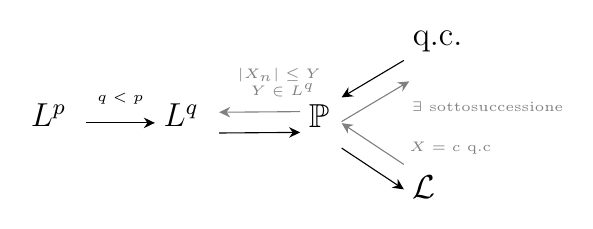
\begin{tikzpicture}[x=0.75pt,y=0.75pt,yscale=-1,xscale=1]
%uncomment if require: \path (0,119); %set diagram left start at 0, and has height of 119

% Text Node
\draw (14,50.4) node [anchor=north west][inner sep=0.75pt]  [font=\large]  {$L^{p}$};
% Text Node
\draw (78,50.4) node [anchor=north west][inner sep=0.75pt]  [font=\large]  {$L^{q}$};
% Text Node
\draw (148,50.9) node [anchor=north west][inner sep=0.75pt]  [font=\large]  {$\PP$};
% Text Node
\draw (198,85.4) node [anchor=north west][inner sep=0.75pt]  [font=\large]  {$\Lc$};
% Text Node
\draw (198,15.4) node [anchor=north west][inner sep=0.75pt]  [font=\large]  {$\text{q.c.}$};
% Text Node
\draw (46,45.4) node [anchor=north west][inner sep=0.75pt]  [font=\tiny]  {$q< p$};
% Text Node
\draw (107,32.9) node [anchor=north west][inner sep=0.75pt]  [font=\tiny,color={rgb, 255:red, 128; green, 128; blue, 128 }  ,opacity=1 ]  {$ \begin{array}{l}
| X_{n}| \leq Y\\
\ \ Y\in L^{q}
\end{array}$};
% Text Node
\draw (197.5,49.5) node [anchor=north west][inner sep=0.75pt]  [font=\tiny,color={rgb, 255:red, 128; green, 128; blue, 128 }  ,opacity=1 ] [align=left] {$\exists $ sottosuccessione};
% Text Node
\draw (196.5,69) node [anchor=north west][inner sep=0.75pt]  [font=\tiny,color={rgb, 255:red, 128; green, 128; blue, 128 }  ,opacity=1 ] [align=left] {$X=c$ q.c};
% Connection
\draw    (42,61) -- (72,61) ;
\draw [shift={(75,61)}, rotate = 180] [fill={rgb, 255:red, 0; green, 0; blue, 0 }  ][line width=0.08]  [draw opacity=0] (5.36,-2.57) -- (0,0) -- (5.36,2.57) -- (3.56,0) -- cycle    ;
% Connection
\draw [color={rgb, 255:red, 128; green, 128; blue, 128 }  ,draw opacity=1 ]   (109,55.86) -- (145,55.58) ;
\draw [shift={(106,55.88)}, rotate = 359.56] [fill={rgb, 255:red, 128; green, 128; blue, 128 }  ,fill opacity=1 ][line width=0.08]  [draw opacity=0] (5.36,-2.57) -- (0,0) -- (5.36,2.57) -- (3.56,0) -- cycle    ;
% Connection
\draw [color={rgb, 255:red, 0; green, 0; blue, 0 }  ,draw opacity=1 ]   (142,65.6) -- (106,65.88) ;
\draw [shift={(145,65.58)}, rotate = 179.56] [fill={rgb, 255:red, 0; green, 0; blue, 0 }  ,fill opacity=1 ][line width=0.08]  [draw opacity=0] (5.36,-2.57) -- (0,0) -- (5.36,2.57) -- (3.56,0) -- cycle    ;
% Connection
\draw    (167.58,47.2) -- (195,30.89) ;
\draw [shift={(165,48.73)}, rotate = 329.25] [fill={rgb, 255:red, 0; green, 0; blue, 0 }  ][line width=0.08]  [draw opacity=0] (5.36,-2.57) -- (0,0) -- (5.36,2.57) -- (3.56,0) -- cycle    ;
% Connection
\draw [color={rgb, 255:red, 128; green, 128; blue, 128 }  ,draw opacity=1 ]   (194.98,42.53) -- (165,60.37) ;
\draw [shift={(197.56,41)}, rotate = 149.25] [fill={rgb, 255:red, 128; green, 128; blue, 128 }  ,fill opacity=1 ][line width=0.08]  [draw opacity=0] (5.36,-2.57) -- (0,0) -- (5.36,2.57) -- (3.56,0) -- cycle    ;
% Connection
\draw [color={rgb, 255:red, 128; green, 128; blue, 128 }  ,draw opacity=1 ]   (167.5,62.79) -- (195,81.04) ;
\draw [shift={(165,61.13)}, rotate = 33.56] [fill={rgb, 255:red, 128; green, 128; blue, 128 }  ,fill opacity=1 ][line width=0.08]  [draw opacity=0] (5.36,-2.57) -- (0,0) -- (5.36,2.57) -- (3.56,0) -- cycle    ;
% Connection
\draw    (192.5,91.38) -- (165,73.13) ;
\draw [shift={(195,93.04)}, rotate = 213.56] [fill={rgb, 255:red, 0; green, 0; blue, 0 }  ][line width=0.08]  [draw opacity=0] (5.36,-2.57) -- (0,0) -- (5.36,2.57) -- (3.56,0) -- cycle    ;

\end{tikzpicture}

\subsection{Proprietà:}

Se $X_n\rightarrow X$ e $Y_n\rightarrow Y$, allora a seconda della convergenza possono valere alcune o tutte le seguenti proprietà:

$1.\ aX_n\rightarrow aX\ \left(\text{qc} ,L^p ,\PP ,\Lc\right)$

$2.\ h( X_n)\rightarrow h(X)\ (\text{qc} ,\PP ,\Lc )$

$3.\ X_n +Y_n\rightarrow X+Y\ \left(\text{qc} ,L^p ,\PP\right)$

$4.\ X_n Y_n\rightarrow XY\ (\text{qc} ,\PP )$

$5.\ Y,Y_n \neq 0\ \forall \omega \Rightarrow \frac{X_n}{Y_n}\rightarrow \frac{X}{Y} \ (\text{qc} ,\PP )$

Se $Y$ converge a una costante in legge valgono anche la $3$, $4$ e $5$ (teorema di Slutsky)
\subsection{LGN:}

Dati $X_n \in L^1$ iid e $\mu \in \RR$, allora $\EE[ X_n] =\mu \Leftrightarrow \overline{X}_n\xrightarrow{\text{qc}} \mu \text{ e }\overline{X}_n\xrightarrow{L^1} \mu $
\subsection{TCL:}

Dati $X_n \in L^2$ iid, $\mu =\EE[ X_n] \ \ \sigma^2 =\Var(X_n) >0$, allora:

$(\overline{X}_n -\mu ) /\left(\frac{\sigma}{\sqrt{n}}\right)\xrightarrow{\Lc} N (0,1)$
\subsection{Velocità di convergenza:}

$X_n$ converge verso $a$ con vel. $v_n$ se: $v_n( X_n -a)\xrightarrow{\Lc} T\nsim \delta_0$
\subsection{Asintotica normalità:}

Se $T\sim \Nc (0,q)$, con $q >0$ allora: $X_n \sim AN\left( a,q/v^2_n\right)$
\subsection{Metodo Delta 1:}

Se $v_n( X_n -a)\xrightarrow{\Lc} T$ allora: $v_n( h( X_n) -h(a))\xrightarrow{\Lc} h'(a)\cdot T$, dove $\Img( X_n) \subseteq B,B$ boreliano di $\RR ,a\in \dot{B}$ (pto. interno), $h:B\rightarrow \RR$ boreliana e diff. in $a$. Nel caso asintot. normale: $X_n \sim AN\left( a,q/v^2_n\right)$

$\Rightarrow h( X_n) \sim AN\left( h(a),\frac{( h'(a))^2 q}{v^2_n}\right)$
\section{Risultati notevoli}
\subsection{Media campionaria:}

$\overline{X}_n =\frac{1}{n}\sum^n_{k=1} X_k$

$1.\ \EE[\overline{X}_n] =\mu \ \ \forall n$ (correttezza)

$2.\ \Var(\overline{X}_n) =\frac{\sigma^2}{n}\xrightarrow{n} 0$ (ovvero $\overline{X}_n\xrightarrow{L^2} \mu $)

$3.\ \overline{X}_n\xrightarrow{\text{qc}} \mu $ per la LGN (consistenza)

$4.\ \frac{\overline{X}_n -\mu}{\sigma /\sqrt{n}}\xrightarrow{\Lc}\Nc (0,1)$ per il TCL.
\subsection{Varianza campionaria:}

$S^2_n =\frac{1}{n-1}\sum^n_{k=1}( X_k -\overline{X}_n)^2$

$1.\ \EE\left[ S^2_n\right] =\sigma^2 \ \ \forall n$ (corretto)

$3.\ S^2_n\xrightarrow{\text{qc}} \sigma^2$ (consistente)

$4.\ \left( S^2_n -\sigma^2\right) /(\sqrt{\frac{\mu_4 -\sigma^4}{n}} )\xrightarrow{\Lc} N (0,1)$

ovvero $S^2_n \sim AN\left( \sigma^2 ,\frac{\mu_4 -\sigma^4}{n}\right)$

dove $\mu_4 =\EE\left[( X_n -\mu )^4\right] \neq \sigma^4$
\subsection{Stima di una proporzione: (corr. e consist.)}

$\hat{p}_n =\frac{1}{n}\sum^n_{k=1}\Ind_B( X_k)$

$(\hat{p}_n -p) /(\sqrt{\frac{p(1-p)}{n}} )\xrightarrow{\Lc} N (0,1)$ per il TCL.
\subsection{Stima della F di ripart.: (corr. e consist.)}

$ \begin{array}{l}
F_n (t)=\frac{1}{n}\sum^n_{k=1}\Ind_{(-\infty ,t)}( X_k)\\
=\frac{1}{n}\sum^n_{k=1}\Ind_{[ X_k ,+\infty )} (t)
\end{array}$

in quanto $X_k \leq t\Leftrightarrow t\geq X_k$

$F_n (t)\sim AN\left( F(t),\frac{F(t)(1-F(t))}{n}\right)$
\subsection{Prodotto di convoluzione:}

$ \begin{array}{l}
Z=X+X,\ P^Z =P^X *P^Y\\
f_Z (z)=( f_X *f_Y) (z)=\int_{\RR} f_{X,Y} (z-y,y)dy
\end{array}$
\subsection{Somma di distribuzioni:}

\textit{Bernoulliane:} $X_1 ,\dotsc ,X_n \sim \Be (p)$ indip.

$\Longrightarrow X_1 +\cdots +X_n \sim \Bi (n,p)$

\textit{Binomiali:} $X_1 \sim \Bi (n_1 ,p),X_2 \sim \Bi (n_2 ,p)$ indip.

$\Longrightarrow X_1 +X_2 \sim \Bi (n_1 +n_2 ,p)$

\textit{Gaussiane:} $X_1 ,\dotsc ,X_n \sim \Nc (0,1)$ indip.

$ \begin{array}{l}
\Longrightarrow X_1 +\cdots +X_n \sim \Nc (0,n)\\
\Longrightarrow X^2_1 +\cdots +X^2_n \sim \chi^2 (n)
\end{array}$

\textit{Esponenziali:} $X_1 ,\dotsc ,X_n \sim \Ec (\lambda )$ indip.

$\Longrightarrow X_1 +\cdots +X_n \sim \Gamma (n,\lambda )$

\textit{Gamma:} $X\sim \Gamma (\alpha ,\lambda ),\ Y\sim \Gamma (\beta ,\lambda )$ indip.

$\Longrightarrow X+Y\sim \Gamma (\alpha +\beta ,\lambda )$

\textit{Poisson:} $X\sim \Pc( \lambda_X) ,\ Y\sim \Pc( \lambda_Y)$ indip.

$\Longrightarrow X+Y\sim \Pc( \lambda_X +\lambda_Y)$
\subsection{Serie:}

$ \begin{array}{l}
\sum^{\infty}_{k=0} q^k =\frac{1}{1-q} ,\ |q|< 1\\
\sum^N_{k=0} q^k =\frac{1-q^{N+1}}{1-q} ,\ |q|< 1\\
e^x =\lim_{n\rightarrow +\infty}\left( 1+\frac{x}{n}\right)^n =\sum^{\infty}_{k=0}\frac{x^k}{k!}\\
\sum^n_{i=1} i=\frac{n(n+1)}{2}\\
\sum^n_{i=1} i^2 =\frac{n(n+1)(2n+1)}{6}\\
\sum^{\infty}_{i=1}\frac{x^i}{i} =\ln\left(\frac{1}{1-x}\right) ,\ |x|\leq 1,\ x\neq 1\\
\sum^n_{i=0}\binom{n}{i} a^{(n-i)} b^i =(a+b)^n\\
\sum^{\infty}_{i=1} ix^i =\frac{x}{(1-x)^2}
\end{array}$
\section{Catene di Markov}
\subsection{Classificazione}

Periodo $d=\MCD\left\{n\geq 1,p^{( n)}_{ii} >0\right\}$

1. Stato aperiodico, se $d=1$ (es. $p_{ii} >0$)

2.a Stato ricorrente, $\PP( \tau_i < +\infty |X_0 =i) =1$, se $p_{ii} =1$ (solo ricciolo) allora anche assorbente

2.b Stato transiente, $\PP( \tau_i < +\infty |X_0 =i) < 1$
\subsection{Chapman-Kolmogorov}

$p^{( n)}_{ij} =\sum\nolimits_k p^{( m)}_{ik} p^{( n-m)}_{kj}$
\subsection{Invariante}

$\sum\nolimits_i \pi_i =1,\pi_i \in [ 0,1] ,\pi =\pi P,\exists $ sempre
\subsection{Risultati utili}

$p^{(k)}_{ij} =\left( P^k\right)_{ij} \ \forall k\in \NN$

CdM \textit{irriducibile:}

- $\exists !\pi ,\ \pi_i =1/\EE_i[ \tau_i]$

- (ergodico1) $\frac{1}{n+1}\sum\nolimits^n_{m=1} h( X_m)\xrightarrow[n]{\text{qc}}\sum\nolimits_{i\in E} h( i) \pi_i \ \forall h:E\rightarrow \RR ,\forall v$

- (ergodico2) $\frac{1}{n+1}\sum\nolimits^n_{m=1}\Ind_{\{i\}}( X_m)\xrightarrow[n]{\text{qc}} \pi_i \ \forall i\in E,\forall v$ (fraz. di tempo che passa in $i$ tra $0$ e $n$ tende alla fraz. che ci passa alla lunga)

se anche \textit{aperiodica}, $v^{( n)}\xrightarrow{n} \pi ,\forall v^{( 0)}$

se \textit{non riducibile}, $\exists \infty \pi $, comb. conv. di ogni $\pi $ di ogni classe chiusa irrid.
\section{Ricorda}

$X$ VA positiva e continua: $\EE[X]=\int\nolimits^{+\infty}_0 (1-F(x))dx$

VA indip. $\Leftrightarrow $ fattorizzano: densità, $\varphi $, $\EE$

Se $(X_1,X_2)$ indip. $\Rightarrow \Cov(X_1,X_2) =0$

Ricondursi ai punti precedenti, usare trasformazioni

Correlazione massima quando c'è al più una densità diversa da $0$ nelle colonne della densità congiunta.
\subsection{Funzione di ripartizione}

$ \begin{array}{l}
F_{\text{max}}( t) =\prod F( t)\\
F_{\text{min}}( t) =1-\prod ( 1-F( t))
\end{array}$


\subsection{Campioni gaussiani}

$X_1 \dotsc X_n$ iid $X_k \sim \Nc\left( \mu ,\sigma^2\right) ,\ \mu \in \RR ,\ \sigma^2 >0$:

1. $\overline{X}_n \sim \Nc\left( \mu ,\sigma^2 /n\right)$

2. $S^2 \sim \frac{\sigma^2}{n-1} \chi^2( n-1)$

3. $\overline{X}_n \Bot S^2$

4. $\frac{\overline{X}_n -\mu}{\sqrt{S^2 /n}} \sim t( n-1)$



\subsection{Convergenza integrali}

$ \begin{array}{l}
\int\nolimits^b_a\frac{1}{( x-a)^p}\rightarrow \begin{cases}
\text{converge} & \text{se} \ p< 1\\
\text{diverge} & \text{se} \ p\geq 1
\end{cases}\\
\int\nolimits^{+\infty}_{\alpha}\frac{1}{x^p}\rightarrow \begin{cases}
\text{converge} & \text{se} \ p >1\\
\text{diverge} & \text{se} \ p\leq 1
\end{cases}
\end{array}$

$ \begin{array}{l}
0< \alpha < 1,\\
\int\limits^{\alpha}_0\frac{1}{x^a| \ln( x)|^b}\rightarrow \begin{cases}
\text{conv.} & \text{se} \ \begin{cases}
a< 1 & \forall b\in \RR\\
a=1 & b >1
\end{cases}\\
\text{div.} & \text{se} \ \begin{cases}
a >1 & \forall b\in \RR\\
a=1 & b\leq 1
\end{cases}
\end{cases}
\end{array}$

$ \begin{array}{l}
\alpha >1,\\
\int\limits^{+\infty}_{\alpha}\frac{1}{x^a(\ln( x))^b}\rightarrow \begin{cases}
\text{conv.} & \text{se} \ \begin{cases}
a >1 & \forall b\in \RR\\
a=1 & b >1
\end{cases}\\
\text{div.} & \text{se} \ \begin{cases}
a< 1 & \forall b\in \RR\\
a=1 & b\leq 1
\end{cases}
\end{cases}
\end{array}$

$ \begin{array}{l}
\alpha >1,\\
\int\limits^{\alpha}_1\frac{1}{(\ln( x))^p}\rightarrow \begin{cases}
\text{converge} & \text{se} \ p< 1\\
\text{diverge} & \text{se} \ p\geq 1
\end{cases}
\end{array}$

\end{multicols}
\end{document}